\documentclass[tikz,border=8pt]{standalone}
\usepackage{tikz}
\usepackage{fontspec}
\setmainfont{DejaVu Sans}
\setsansfont{DejaVu Sans}
\usetikzlibrary{arrows.meta, positioning, shapes.geometric, calc, fit, backgrounds}
\begin{document}
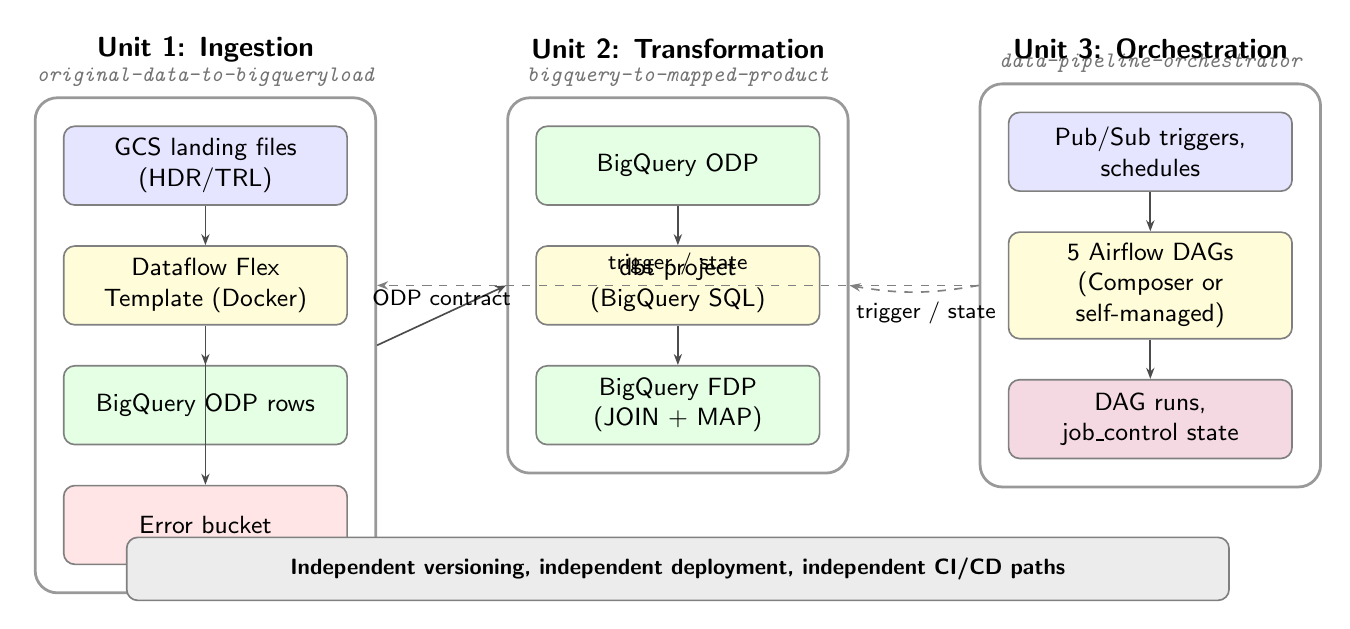
\begin{tikzpicture}[
  font=\sffamily\small,
  every node/.style={font=\sffamily\small},
  box/.style={draw=black!50, line width=0.6pt, rounded corners=4pt, minimum width=2.4cm, minimum height=1cm, align=center, inner sep=4pt},
  src/.style={box, fill=blue!10},
  storage/.style={box, fill=green!10},
  compute/.style={box, fill=yellow!15},
  output/.style={box, fill=purple!15},
  control/.style={box, fill=gray!15, font=\sffamily\footnotesize\itshape},
  err/.style={box, fill=red!10},
  arrow/.style={-{Stealth[length=4pt]}, line width=0.6pt, draw=black!70},
  dashed-arrow/.style={arrow, dashed, draw=black!50},
  caption/.style={font=\sffamily\footnotesize, text=black!60},
  unitbox/.style={draw=black!40, line width=1pt, rounded corners=8pt, inner sep=10pt},
  unitlabel/.style={font=\sffamily\footnotesize\itshape, text=black!55}
]

% === UNIT 1: INGESTION ===
\node[compute, minimum width=3.6cm] (df1) at (0,0) {Dataflow Flex\\Template (Docker)};
\node[src, minimum width=3.6cm, above=0.5cm of df1]  (inp1) {GCS landing files\\(HDR/TRL)};
\node[storage, minimum width=3.6cm, below=0.5cm of df1] (out1a) {BigQuery ODP rows};
\node[err,     minimum width=3.6cm, below=0.5cm of out1a] (out1b) {Error bucket};

\draw[arrow] (inp1) -- (df1);
\draw[arrow] (df1)  -- (out1a);
\draw[arrow] (df1)  -- (out1b);

\begin{scope}[on background layer]
  \node[unitbox, fit=(inp1)(df1)(out1a)(out1b), label={[unitlabel]above:\texttt{original-data-to-bigqueryload}}] (u1) {};
\end{scope}
\node[font=\sffamily\normalsize\bfseries] at (0, 3.0) {Unit 1: Ingestion};

% === UNIT 2: TRANSFORMATION ===
\node[compute, minimum width=3.6cm] (dbt2) at (6,0) {dbt project\\(BigQuery SQL)};
\node[storage, minimum width=3.6cm, above=0.5cm of dbt2] (inp2) {BigQuery ODP};
\node[storage, minimum width=3.6cm, below=0.5cm of dbt2] (out2) {BigQuery FDP\\(JOIN + MAP)};

\draw[arrow] (inp2) -- (dbt2);
\draw[arrow] (dbt2) -- (out2);

\begin{scope}[on background layer]
  \node[unitbox, fit=(inp2)(dbt2)(out2), label={[unitlabel]above:\texttt{bigquery-to-mapped-product}}] (u2) {};
\end{scope}
\node[font=\sffamily\normalsize\bfseries] at (6, 3.0) {Unit 2: Transformation};

% === UNIT 3: ORCHESTRATION ===
\node[compute, minimum width=3.6cm] (af3) at (12,0) {5 Airflow DAGs\\(Composer or\\self-managed)};
\node[src,     minimum width=3.6cm, above=0.5cm of af3]  (inp3) {Pub/Sub triggers,\\schedules};
\node[output,  minimum width=3.6cm, below=0.5cm of af3] (out3) {DAG runs,\\job\_control state};

\draw[arrow] (inp3) -- (af3);
\draw[arrow] (af3)  -- (out3);

\begin{scope}[on background layer]
  \node[unitbox, fit=(inp3)(af3)(out3), label={[unitlabel]above:\texttt{data-pipeline-orchestrator}}] (u3) {};
\end{scope}
\node[font=\sffamily\normalsize\bfseries] at (12, 3.0) {Unit 3: Orchestration};

% === ARROWS BETWEEN UNITS ===
% ODP contract: Unit1 -> Unit2
\draw[arrow] (u1.east) -- node[above, font=\sffamily\footnotesize] {ODP contract} (u2.west);

% trigger/state: Unit3 -> Unit1
\draw[dashed-arrow] (u3.west) to[out=180,in=0] node[above, font=\sffamily\footnotesize, pos=0.5] {trigger / state} (u1.east |- u3.west);
% trigger/state: Unit3 -> Unit2
\draw[dashed-arrow] (u3.west) to[out=190,in=350] node[below, font=\sffamily\footnotesize, pos=0.4] {trigger / state} (u2.east);

% === BOTTOM BAR ===
\node[control, minimum width=14cm, minimum height=0.8cm] at (6,-3.6)
  {\textbf{Independent versioning, independent deployment, independent CI/CD paths}};

\end{tikzpicture}
\end{document}
